\chapter{Ideal Fluids}

\section{Describing Ideal Flow}

There are often situations where the viscosity of a fluid is unimportant -- for example, in high Reynolds number flow.  In those cases we can set the viscosity to zero and the fluid is called \emph{inviscid}.  If we also keep our flow incompressible (so that the density is constant throughout the fluid) then the fluid is \emph{ideal}.  Of course, real fluids always have \emph{some} viscosity; however, as discussed in Section \ref{sec_viscosity}, in many cases an ideal fluid can be a good approximation to a real one.  Keep in mind, however, that the boundary layer present in viscous fluids can never be described by an ideal fluid, so we'll miss some of the physics due to that.

Under these assumptions, the Navier-Stokes equation is usually called \emph{Euler's equation},
\begin{equation}
\label{eq_euler}
\boxed{
\frac{D \uu}{Dt} = -\frac{1}{\rho} \grad p + \symbfup{g}.
}
\end{equation}
The incompressibility condition,
\begin{equation}
\grad \cdot \uu = 0,
\end{equation}
remains the same.



\subsection{Static Fluids}
\label{sec_static}

The simplest solution to Euler's equation (and, in fact, the Navier-Stokes equation) is the trivial one:  suppose the fluid is at rest, so that $\uu = \vec{0}$ everywhere.  Then equation \ref{eq_euler} reduces to 
\[
\vec{0} = -\frac{1}{\rho} \grad p + \symbfup{g},
\]
or 
\[
\grad p = \rho \symbfup{g}.
\]
If we take the direction of gravity to be down as usual, so that $\symbfup{g} = [0,0,-g]$, this equation says
\[
\frac{\partial p}{\partial x} = 0, \quad \frac{\partial p}{\partial y} = 0, \quad \frac{\partial p}{\partial z} = -\rho g.
\]
The first two equations just say that the pressure $p$ doesn't depend explicitly on $x$ or $y$, and we can integrate the third to get
\begin{equation}
p = p_0 - \rho g z,
\end{equation}
where $p_0$ is the integration constant.  If our fluid has a ``free surface'' -- that is, it's open to the atmosphere -- at $z=0$, then $p_0$ is the atmospheric pressure.

This result is simple and tells us what we already know from experience:  as you go down in depth ($z < 0$) in a fluid, the pressure increases.  Note, however, that we've assumed the density $\rho$ stays constant; in some fluids (like the atmosphere) it's a bad assumption, while in others (like the ocean, at least for reasonable depths) it's okay.




\subsection{Bernoulli's Principle}

Since gravity is a conservative force, we can always write it in terms of the gradient of a scalar, so that
\[
\symbfup{g} = - \grad \Phi,
\]
where $\Phi$ is called the gravitational potential.  For example, setting $\Phi = gz$ gives us our usual $\symbfup{g}$ pointing down along the $z$ axis.

With this change, Euler's equation becomes
\begin{equation}
\frac{\partial \uu}{\partial t} + (\uu \cdot \grad) \uu = -\grad \left( \frac{p}{\rho} + \Phi \right).
\label{eq_euler_bern}
\end{equation}
It turns out that the second term on the left can be written as (see Problem \ref{prob_vc3})
\begin{equation}
 (\uu \cdot \grad) \uu = (\curl \uu ) \times \uu + \grad (\tfrac{1}{2} \uu^2),
\end{equation}
where $\uu^2 = \uu \cdot \uu$; as usual, be careful of all the different $u$s we deal with.  With this substitution, and moving the gradient onto the right hand side, Euler's equation is now
\begin{equation}
\label{eq_euler_bernoulli}
\frac{\partial \uu}{\partial t} + (\curl \uu ) \times \uu = -\grad \left( \frac{p}{\rho} + \tfrac{1}{2} \uu^2 + \Phi \right).
\end{equation}

This doesn't look any better than the original form of Euler's equation, though.  We can clean it up a bit by defining
\[
H \equiv \frac{p}{\rho} + \tfrac{1}{2} \uu^2 + \Phi,
\]
which is sometimes called the ``total head'' or ``energy head'' of the flow.  If we also assume the flow is \emph{steady}, we then have
\begin{equation}
(\curl \uu ) \times \uu = -\grad H.
\label{eq_bernoulli}
\end{equation}
One last step -- take the dot product with $\uu$ for both sides:
\[
\uu \cdot [(\curl \uu ) \times \uu] = -\uu \cdot \grad H.
\]
But now the left hand side is zero -- the term in the square brackets has a direction perpendicular to $\uu$, so the dot product with $\uu$ vanishes.  So we're left with
\begin{equation}
\boxed{
(\uu \cdot \grad) H  = 0.
}
\end{equation}
As we learned back in Section \ref{sec_tot_deriv}, this means that the quantity $H$ is \emph{constant along a streamline} for steady flow.  This is \emph{Bernoulli's streamline theorem.}

If the fluid is also irrotational, so that $\curl \uu = 0$, equation (\ref{eq_bernoulli}) gives us the stronger statement
\begin{equation}
\boxed{
\grad H = 0,
}
\end{equation}
so that $H$ is constant everywhere in the fluid.

\begin{figure}
\centering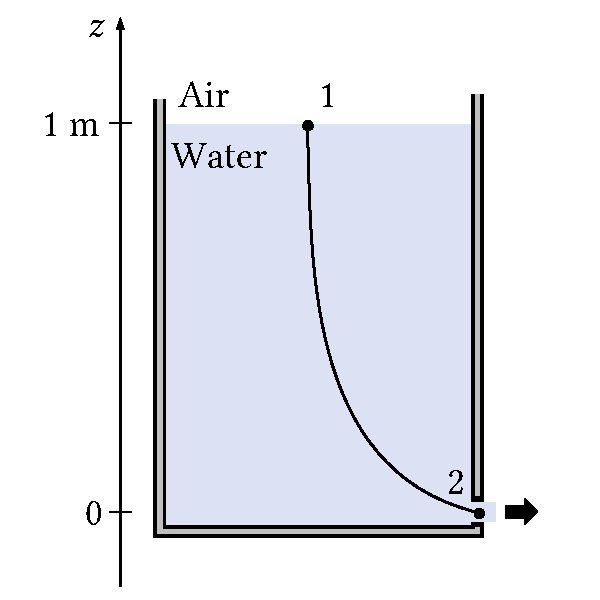
\includegraphics[width=0.5\linewidth]{Figures/Chapter3/fig_leaky_bucket}
\caption{A large tank of water has sprung a leak.  How fast is the water moving as it comes out of the hole?}
\label{fig_leaky_bucket}
\end{figure}

\begin{example}[A leaky bucket]
A large tank of water, open to the atmosphere at the top, suddenly springs a leak near the bottom (see Figure \ref{fig_leaky_bucket}).  If the hole is 1.0 m below the free surface, what is the speed of the water as it comes out the hole?

This is a good case for Bernoulli's principle, since the flow is (approximately) steady -- the surface will drop only slowly if the hole is small.  We can therefore use the streamline theorem:
\[
H = \frac{p}{\rho} + \tfrac{1}{2} \uu^2 + gz = \text{constant}.
\]
Presumably there exists a streamline that connects the free surface at the top of the tank with the hole (joining points 1 and 2 as shown in Figure \ref{fig_leaky_bucket}).  Then we can evaluate $H$ at both points:
\begin{itemize}
\item Point 1 $\to H_1 = \frac{p_1}{\rho} + \tfrac{1}{2} \uu_1^2 + gz_1$
\item Point 2 $\to H_2 = \frac{p_2}{\rho} + \tfrac{1}{2} \uu_2^2 + gz_2$
\end{itemize}
But $p_1 = p_2 = p_0$ since both locations are open to the atmosphere.  We'll also take $\uu_1 = 0$, since the surface drops only very slowly.  Finally, using the coordinate system shown in Figure \ref{fig_leaky_bucket}, we have $z_2 = 0$ (and $z_1 = 1$ m).

Setting $H_1 = H_2$ then gives us
\[
\frac{p_0}{\rho} + gz_1 = \frac{p_0}{\rho} + \tfrac{1}{2} \uu_2^2.
\]
The pressure terms cancel, and we can rearrange for the speed of the water:
\[
|\uu| = \sqrt{2gz_1} \approx 4.4 \text{ m/s}.
\]
\end{example}






\subsection{The Vorticity Equation}
\label{sec_vorticity_eq}

Let's rewrite Euler's equation again, this time in terms of the vorticity.  Going back to equation (\ref{eq_bernoulli}) and writing $\vort = \curl \uu$, we have
\[
\frac{\partial \uu}{\partial t} + \vort \times \uu = -\grad H.
\]
Take the curl of both sides:
\begin{equation}
\frac{\partial \vort}{\partial t} + \curl (\vort \times \uu) = -\curl \grad H.
\label{eq_curl_euler}
\end{equation}
But the curl of a gradient is identically zero (see Problem \ref{prob_vc2}), so the right hand side vanishes.

Now, there's a vector identity (another one!) that says, for two vectors $\symbfup{F}$ and $\symbfup{G}$,
\begin{equation}
\curl (\symbfup{F} \times \symbfup{G}) = (\symbfup{G} \cdot \grad) \symbfup{F} - (\symbfup{F} \cdot \grad) \symbfup{G} + \symbfup{F} (\symbfup{\nabla} \cdot \symbfup{G}) - \symbfup{G} (\symbfup{\nabla} \cdot \symbfup{F})
\end{equation}
(see Problem \ref{prob_vc4}).  Using this in equation \ref{eq_curl_euler} above, with $\vort$ replacing $\vec{F}$ and $\uu$ replacing $\symbfup{G}$, gives us
\[
\frac{\partial \vort}{\partial t} + (\uu \cdot \grad) \vort - (\vort \cdot \grad)\uu + \vort (\symbfup{\nabla} \cdot \uu) - \uu(\symbfup{\nabla} \cdot \vort) = 0.
\]
Of course, we're dealing with an ideal fluid, so $\symbfup{\nabla} \cdot \uu = 0$, and, since $\vort$ is a curl, $\symbfup{\nabla} \cdot \vort = 0$ identically (see Problem \ref{prob_vc2} again for that one).  So the fourth and fifth terms vanish, and we have
\[
\frac{\partial \vort}{\partial t} + (\uu \cdot \grad) \vort = (\vort \cdot \grad)\uu.
\]
Finally, we can combine the two terms on the right hand side -- that's the definition of the material derivative of $\vort$ -- and we have, at long last, the \emph{vorticity equation},
\begin{equation}
\label{eq_vorticity}
\boxed{
\frac{D \vort}{Dt} = (\vort \cdot \grad) \uu.
}
\end{equation}

This equation will prove useful every once in a while for us.  In particular, for a two dimensional flow, where 
\[
\vort = [0,0,\omega],
\]
it's easy to see that the right hand side becomes zero, and we end up with
\begin{equation}
\frac{D \vort}{Dt} = 0.
\end{equation}
This means that the vorticity of each individual fluid element is conserved, a result we'll use later.  Furthermore, if the flow is also steady, this becomes
\begin{equation}
(\uu \cdot \grad) \omega = 0,
\end{equation}
and the vorticity is constant along streamlines in this case.



\subsection{Circulation}
\label{sec_circulation}

\begin{figure}
\centering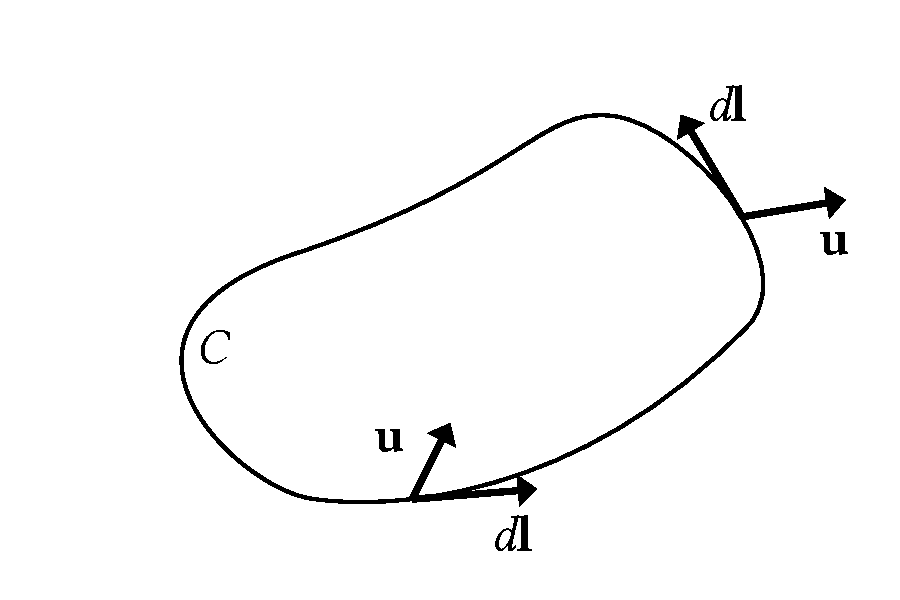
\includegraphics[width=0.5\linewidth]{Figures/Chapter3/fig_circ}
\caption{A closed curve $C$ lies within the fluid region.}
\label{fig_circ}
\end{figure}

Consider a closed curve $C$ that lies in the fluid region as shown in Figure \ref{fig_circ}.  The circulation $\Gamma$ is defined as the line integral
\begin{equation}
\boxed{
\Gamma = \oint_C \uu \cdot d\vec{l}.
}
\label{eq_circ}
\end{equation}
Notice the role the dot product plays in the integral -- as we go around the curve, only the fluid velcity that points in the direction of the curve is added, giving us the fluid that is circulating around that curve.

\begin{example}[Line Vortex]
We've explored the flow around a line vortex before -- its vorticity in Example \ref{ex_vorticity_line_vortex} and its generation in Section \ref{sec_line_vortex} -- and we'll see it again later on.  Now let's find the circulation around it.

The flow is given by
\[
\vec{u} = \frac{\Gamma_0}{2\pi s} \, \unit{\phi},
\]
and to calculate the circulation we'll use a circular path of constant radius $R$.  The dot product in the integral becomes
\[
\vec{u} \cdot d\vec{l} = \left( \frac{\Gamma_0}{2\pi s} \, \unit{\phi} \right) \cdot \left( ds \, \unit{s} + s d\phi \, \unit{\phi} + dz \, \unit{z} \right),
\]
where we evaluate $\vec{u}$ and $d\vec{l}$ aloing the curve, and get
\[
\vec{u} \cdot d\vec{l} = \frac{\Gamma}{2\pi}.
\]
The circulation is then
\[
\Gamma = \oint_0^{2\pi} \frac{\Gamma_0}{2\pi} \, d\phi = \Gamma_0.
\]
So the line vortex has \emph{constant} circulation with strength given by $\Gamma_0$.
\end{example}

We can write the defintion of the circulation in a different way using Stokes' theorem:
\begin{equation}
\label{eq_circ_curl}
\Gamma = \oint_C \vec{u} \cdot d\vec{l} = \int_S (\grad \times \vec{u} ) \cdot d\vec{a},
\end{equation}
where $S$ is the surface inside the closed curve with area vector $d\vec{a}$.  Now, if $\grad \times \vec{u} = \vec{0}$, then $\Gamma = 0$ as well, which means that the circulation is zero inside any irrotational flow.  However, this is only true if the fluid is \emph{everywhere} irrotational; in particular, if there is an object (like a cylinder or an airplane wing, both examples we'll be doing soon), Stokes' theorem fails and it \emph{is} possible to have circulation in the fluid.

What if we suppose the closed curve actually moves with the fluid -- so that the curve always constists of the same fluid elements?  You can visualize this by prentending we put a bit of food colouring along the curve, so that as the fluid moves about and the curve changes shape, so too will the colouring -- but it will always remain a close curve.  We'll denote the curve now as $C(t)$ to indicate its dependence on time.  

Now, \emph{Kelvin's circulation theorem} says that the circulation $\Gamma$ around $C(t)$ is \emph{independent} of time -- no matter how it changes as the fluid moves, $\Gamma$ stays the same value.  This is an important theorem, especially for understanding lift, so let's go through the proof.

Start with the time derivative of the circulation,
\[
\frac{d\Gamma}{dt} = \frac{d}{dt} \left( \oint_{C(t)} \uu \cdot d\vec{l} \right),
\]
and move the derivative into the integral.  Careful though -- this is the \emph{total} time derivative, and becomes the material derivative inside:
\[
\frac{d\Gamma}{dt} = \oint_{C(t)} \frac{D\vec{u}}{Dt} \cdot d\vec{l}.
\]
But from equation (\ref{eq_euler_bern}) we can write 
\[
\frac{D\vec{u}}{Dt} = -\grad \left(\frac{p}{\rho} + \Phi \right),
\]
so
 \[
\frac{d\Gamma}{dt} = \oint_{C(t)} \grad \left.  \left(\frac{p}{\rho} + \Phi \right) \cdot d\vec{l} = - \left(\frac{p}{\rho} + \Phi \right) \right|_{C(t)}.
\]

We now have to evaluate the pressure, density, and graviational potential along the curve $C(t)$ -- but this is a closed curve and the integration takes us back to the starting point.  Since all three quantities are single-valued functions, they have the same value at the start and end of the curve -- so we get 
\begin{equation}
\frac{d\Gamma}{dt} = 0.
\end{equation}

This result is actually very general -- the fluid could be viscous and could have holes; as long as $C(t)$ moves with the fluid the circulation along it will be constant.





\subsection{The Surface of a Rotating Fluid}

Let's end this section with a classic problem involving ideal fluids: the spinning water bucket example.  In short, we'll fill a bucket with water and start rotating the bucket, letting it come to a steady state.  We solved this problem already back in Section \ref{sec_uni_rot_fluid}, where we found the steady state of the fluid was described by the velocity
\[
\uu = \Omega s \, \unit{\phi},
\]
where $\Omega$ was the angular speed of the rotating boundary -- the bucket in this case -- and the rotation was about the $z$ axis.  Converting this to Cartesian coordinates gives us
\begin{equation}
\label{eq_bucket_vel}
\uu = [-\Omega y, \Omega x, 0].
\end{equation}

Now, we \emph{found} this velocity from the Navier-Stokes equation, and viscosity is important in getting the fluid into rotation in the first place, but once steady-state has been reached, the viscosity is no longer important and the fluid can be treated as ideal.  We can thus examine the flow further using only Euler's equation rather than the full Navier-Stokes.

If you look at a good photograph of this, you'll see that the surface of the water is \emph{curved} (Figure \ref{fig_bucket}).  What is the shape of this free surface?  Well, the thing that all fluid elements along the free surface have in common is that they have the same pressure -- namely, since they're at the surface, atmospheric pressure $p_0$.  Let's find the pressure in the water, then.

\begin{figure}[t]
\centering\includegraphics[width=0.7\linewidth]{Figures/Chapter3/fig_water_bucket.jpg}
\caption{A tank of water is smoothly spun up, causing the water to ``climb'' the sides of the tank.}
\label{fig_bucket}
\end{figure}

The $x$ component of Euler's equation, with $\symbfup{g} = [0,0,-g]$, is
\[
\frac{\partial u}{\partial t} + u\frac{\partial u}{\partial x} +  v\frac{\partial u}{\partial y} + w\frac{\partial u}{\partial z} = -\frac{1}{\rho} \frac{\partial p}{\partial x}.
\]
But the flow is \emph{steady}, and $u$ doesn't depend on $x$ or $z$.  Substituting in the fluid velocity in equation (\ref{eq_bucket_vel}), this equation reduces to
\begin{equation}
\label{eq_px}
\frac{\partial p}{\partial x} = \rho \Omega^2 x.
\end{equation}
Similarly, the $v$ and $w$ equations reduce to
\begin{equation}
\label{eq_py}
\frac{\partial p}{\partial y} = \rho \Omega^2 y
\end{equation}
and
\begin{equation}
\label{eq_pz}
\frac{\partial p}{\partial z} = -\rho g.
\end{equation}

We can now integrate to find the pressure $p(x, y, z)$.  From equation (\ref{eq_px}) we get
\[
p = \tfrac{1}{2} \rho \Omega^2 x^2 + f(y, z),
\]
where the function $f(y,z)$ is there since equation (\ref{eq_px}) is a \emph{partial} derivative -- we don't just get a constant of integration, but a possible function of the other two variables.  Integrating equation (\ref{eq_py}) gives
\[
p = \tfrac{1}{2} \rho \Omega^2 y^2 + g(x, z),
\]
and integrating equation (\ref{eq_pz}) gives
\[
p = -\rho g z + h(x, y).
\]
By inspection, it's clear that the pressure must be
\[
p(x, y, z) = \tfrac{1}{2} \rho \Omega^2 (x^2 + y^2) - \rho gz + p_1,
\]
where $p_1$ is a constant -- it's the pressure at the origin where $x=y=z=0$.

That's the pressure everywhere in the water.  To find the shape of the free surface, we'll set $p = p_0$ and solve for the height $z$:
\begin{equation}
z = \frac{\Omega^2}{2g} (x^2 + y^2) + \left( \frac{p_1 - p_0}{\rho g} \right).
\end{equation}
This is a \emph{paraboloid} -- see Figure \ref{fig_bucket_para} -- and it matches the shape in the photograph in Figure \ref{fig_bucket}.

\begin{figure}
\centering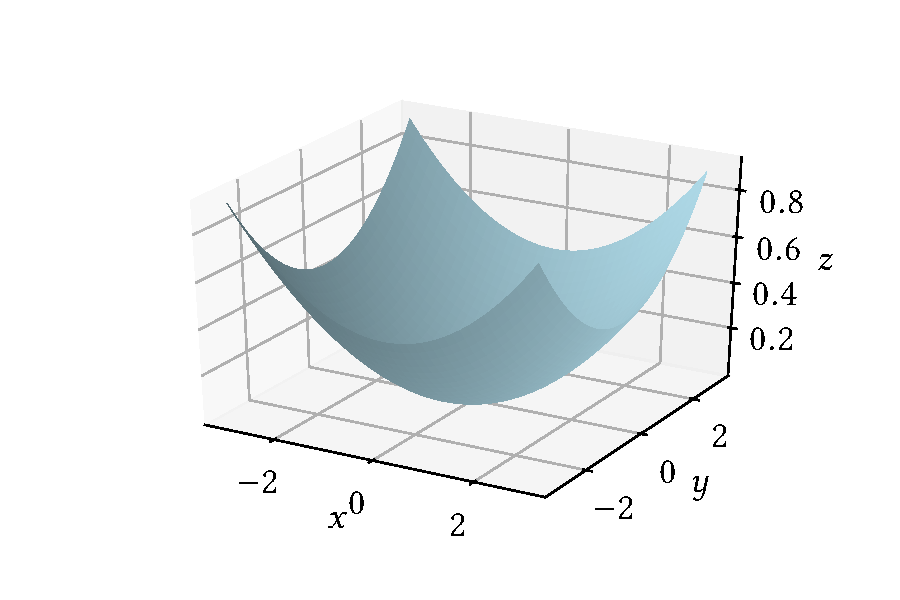
\includegraphics[width=0.8\linewidth]{Figures/Chapter3/fig_paraboloid}
\caption{The free surface of the spinning bucket problem is a paraboloid. }
\label{fig_bucket_para}
\end{figure}





\section{The Velocity Potential and Stream Function}

\subsection{The Velocity Potential}

For any irrotational flow, where
\[
\curl \uu = \vec{0},
\]
a scalar function $\varphi$ can be defined such that
\begin{equation}
\label{eq_vel_pot}
\boxed{
\uu = \grad \varphi.
}
\end{equation}
Then, since the curl of a gradient is zero, irrotationality is automatically satisfied. The quantity $\varphi$ is called the \emph{velocity potential}.  In addition, from Stokes' theorem, we also have that
\[
\oint \uu \cdot d\vec{l} = \int (\curl \uu) \cdot d\vec{a} = 0,
\]
so that the line integral of $\vec{u}$ around any closed loop in the fluid is zero.  This suggests we could also write the velocity potential as
\begin{equation}
\label{eq_vel_pot2}
\varphi(\vec{r}) = \int_{\mathcal{O}}^{\vec{r}} \uu \cdot d\symbfup{l},
\end{equation}
where $\mathcal{O}$ is an arbitrary point in the fluid.  Incidentally, sorry for the notation -- I'm using the Greek letter phi for three things:  the gravitational potential $\Phi$, the cylindrical coordinate $\phi$, and now the velocity potential $\varphi$.  I hope it's not too confusing in context.

This might be familiar to you from electrostatics, where the electric field is also irrotational and we can define an electric potential.  There's a subtle point that frequently arises in fluid dynamics, though, so be careful.  As long as the region is \emph{simply connected} -- that is, the fluid has no holes in it -- the path between $\mathcal{O}$ and $\vec{r}$ doesn't matter, and this leads to $\varphi$ being a single-valued function.  However, if the region is \emph{multiply connected} -- it has holes, regions where there is no fluid -- the integral \emph{could} depend on the path and $\varphi$ will be a multivalued function of position.  This can happen if the fluid is surrounding an object, something we'll start to encounter more frequently.  Let's investigate this in more detail with two examples.

\begin{example}[Flow past a stagnation point]
\label{ex_stag_pot}
Recall the flow past a stagnation point (from Examples \ref{ex_stag_point1} to \ref{ex_stag_point2}), given by
\[
\uu = [\alpha x, -\alpha y, 0].
\]
This is irrotational flow (but check to be sure!), and to find the velocity potential, we write
\[
\frac{\partial \varphi}{\partial x} = u = \alpha x \quad \text{and} \quad \frac{\partial \varphi}{\partial y} = v = -\alpha y.
\]
Integrating each term and combining gives
\[
\varphi(x, y) = \tfrac{1}{2} \alpha (x^2 - y^2) + c,
\]
where $c$ is the integration constant.  However, since it's the fluid velocity, not the potential, that is the physically meaningful quantity, we can set the constant $c$ to zero without losing anything -- after all, we'll take a derivative of $\varphi$ to get the velocity, and the constant will end up going away anyway.

Note that, in this example, $\varphi$ is a single-valued function of $x$ and $y$.  That means that, for any point in the fluid, $\varphi$ has a single value.  This might not always be the case, as our next example will show.
\end{example}

\begin{example}[Line vortex flow]
\label{ex_pot_vortex}
Next, consider the flow
\[
\uu = \frac{\Gamma}{2\pi s} \, \unit{\phi}.
\]
This is the flow around a line vortex, which we've also seen before.  We have to be a bit more careful for this flow -- it's irrotational (we showed that back in Problem \ref{prob_vortex_vorticity}), but not at the origin where it blows up.  To fix this problem, we'll suppose there's \emph{no} fluid there -- maybe there's a cylinder of radius $a$ there instead, covering up the problem area.  That means the fluid domain is $s \ge a$, but it also means there's now a hole in the fluid domain; it's multiply connected.

The potential is found from equation (\ref{eq_vel_pot}) as usual, but in cylindrical coordinates it looks like
\[
\frac{\partial \varphi}{\partial s} = u_s = 0, \quad \frac{1}{s} \frac{\partial \varphi}{\partial \phi} = u_\phi = \frac{k}{s}, \quad \text{and} \quad \frac{\partial \varphi}{\partial z} = u_z = 0.
\]
Integrating this gives
\begin{equation}
\varphi(\phi) = k \phi.
\end{equation}
But note that this isn't a single-valued function -- $\varphi$ has different values at the same point in space:  $\varphi(0) = 0$, but $\varphi(2\pi) = 2\pi k$, and so on.  We'll see later on that this is connected to circulation within the fluid.

\end{example}

Finally, if the fluid is both irrotational \emph{and} incompressible, it must also satisfy the incompressibility condition,
\[
\symbfup{\nabla} \cdot \uu = 0.
\]
If we rewrite this in terms of the potential, we get
\[
\symbfup{\nabla} \cdot \grad \varphi = 0,
\]
or
\begin{equation}
\boxed{
\nabla^2 \varphi = 0.
}
\end{equation}
This is \emph{Laplace's equation}; any irrotational, incompressible fluid must satisfy it.





\subsection{Flow Past a Cylinder}
\label{sec_cylinder}

Working with the velocity potential rather than the velocity itself is often easier; not only is a scalar function easier to work with than a vector field, but Laplace's equation can be easier to solve than Euler's equation, which also contains the pressure of the fluid as an unknown.  As an example of solving Laplace's equation, we'll find the ideal flow past a cylinder oriented perpendicular to the flow.

We'll start with a few basic assumptions.  First, we'll treat this as two dimensional flow, which means the cylinder is effectively infinitely long.  We'll put the cylinder, which has a radius $a$, along the $z$-axis, and the flow will be uniform in the $x$-direction infinitely far away from the cylinder (see Figure \ref{fig_cyl_setup2}):
\begin{equation}
\label{eq_uniform}
\uu (\infty) = U \, \unit{x},
\end{equation}
where $U$ is the constant speed of the flow far away from the cylinder.

\begin{figure}
\centering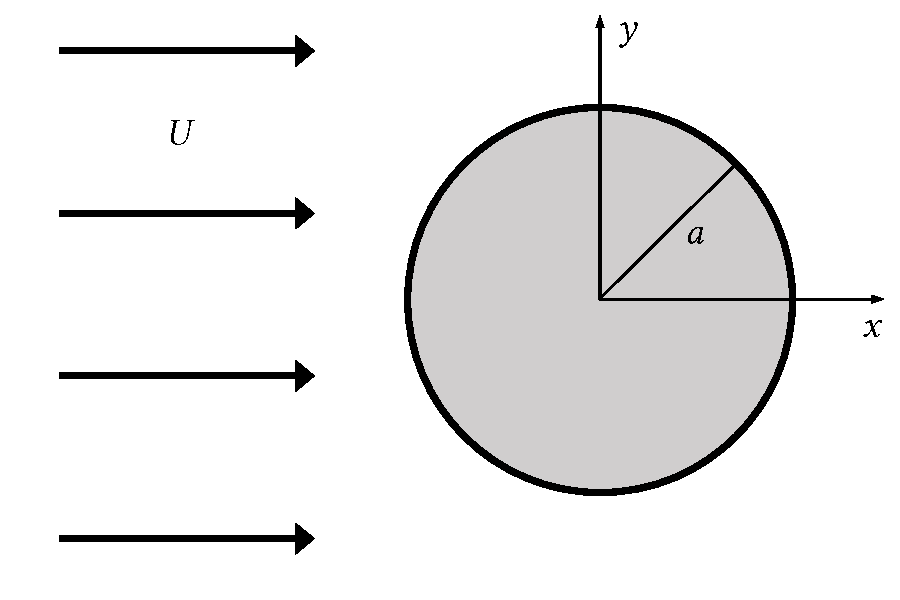
\includegraphics[width=0.7\linewidth]{Figures/Chapter3/fig_cyl_setup}
\caption{Fluid flows past the cylinder along the $x$-direction.}
\label{fig_cyl_setup2}
\end{figure}

The other assumption we'll make is that the flow is irrotational.  This seems like a leap to make, though, since we don't even know what the flow \emph{is} yet.  But remember the vorticity equation (equation \ref{eq_vorticity}) -- for a steady two dimensional flow, the vorticity is conserved along streamlines.  Since the vorticity at infinity, where the flow is \emph{uniform}, is definitely zero, and every streamline starts and ends at infinity, it follows that the flow is everywhere irrotational.

Wait, is our flow \emph{steady}?  Yes, as long as we examine the problem from the point of view that the flow has been happening for a while and reached a steady state.  In practice, it doesn't take long for the fluid to do this.

To find the fluid velocity around the cylinder, we'll solve Laplace's equation.  It makes sense to use cylindrical coordinates here, given the symmetry of the boundary.  In cylindrical coordinates, then, Laplace's equation is
\begin{equation}
\label{eq_laplace_cyl}
\ddfdx{\varphi}{s} + \frac{1}{s} \dfdx{\varphi}{s} + \frac{1}{s^2} \ddfdx{\varphi}{\phi} + \ddfdx{\varphi}{z} = 0.
\end{equation}
Of course, we're assuming a two dimensional flow, so the $z$ term we can safely ignore.

Our boundary conditions are straightforward to write down.  First, as $s \to \infty$, we should have the uniform flow given by equation (\ref{eq_uniform}).  But we need the potential rather than the velocity; following similar steps as in the examples above, the potential for uniform flow along the $x$-direction is
\begin{equation}
\label{eq_cyl_bc1}
\varphi = Ux = U s \cos \phi,
\end{equation}
where I've converted the Cartesian coordinates to cylindrical.  Our first boundary condition, then, is that the flow must become this as $s \to \infty$.

Secondly, at $s=a$, we have the actual boundary.  Unlike viscous flows, ideal fluids must ``slip'' along a boundary; in this case, that means we must have the fluid velocity at $s=a$ be purely in the $\unit{\phi}$ direction.  In other words, we need $u_s = 0$; in terms of the potential (using the gradient in cylindrical coordinates), that's
\begin{equation}
\label{eq_cyl_bc2}
\dfdx{\varphi}{s} = 0 \quad \text{at} \quad s=a.
\end{equation}

We'll solve Laplace's equation using separation of variables.  Let
\[
\varphi(s, \phi) = S(s) \Phi(\phi).
\]
Then equation (\ref{eq_laplace_cyl}) becomes
\[
\Phi \frac{d^2S}{ds^2} + \frac{\Phi}{s} \frac{dS}{ds} + \frac{S}{s^2} \frac{d^2 \Phi}{d\phi^2} = 0,
\]
or, dividing by $S\Phi$ and multiplying by $s^2$,
\begin{equation}
\label{eq_cyl_sep}
\frac{s^2}{S} \frac{d^2S}{ds^2} + \frac{s}{S} \frac{dS}{ds} = -\frac{1}{\Phi} \frac{d^2 \Phi}{d \phi^2}.
\end{equation}
The left hand side of the equation is a function of $s$ only, while the right hand side is a function of $\phi$ only; they must therefore both be equal to a constant.  We'll call the this separation constant $k^2$.  The $\phi$ equation is then
\[
\frac{d^2 \Phi}{d\phi^2} = -k^2 \Phi,
\]
which has the solution
\[
\Phi (\phi) = A \sin k\phi + B \cos k\phi.
\]

We can apply our first boundary condition, equation (\ref{eq_cyl_bc1}), right away to eliminate the sine term, since we need only a cosine dependence as $s \to \infty$.  Comparing the form of equation (\ref{eq_cyl_bc1}) with our solution, we furthermore must have $k=1$.  Thus 
\begin{equation}
\Phi(\phi) = B \cos \phi.
\end{equation}

The radial part of equation (\ref{eq_cyl_sep}) (with $k = 1$) now reads
\[
s^2 \frac{d^2S}{ds^2} + s \frac{dS}{ds} - S = 0.
\]
We've seen this differential equation before; it can solved by trying a power-law solution of the form $S(s) = s^m$.  The general solution is
\[
S(s) = Cs + \frac{D}{s}.
\]
But our second boundary condition, equation (\ref{eq_cyl_bc2}), was that the first derivative of the potential goes to zero at $s=a$.  That means
\[
\frac{dS}{ds} = \left. \left( C - \frac{D}{s^2} \right)  \right|_{s=a} = 0,
\]
and so $D = a^2 C$.

Combining the radial and angular equations gives us
\[
\varphi(s, \phi) = S(s) \Phi(\phi) = C \left( s+\frac{a^2}{s} \right) \cos \phi,
\]
where I absorbed the constants into $C$.  One more comparison with our boundary condition, equation (\ref{eq_cyl_bc1}), tells us that $C = U$.  So our solution to Laplace's equation is, finally, 
\begin{equation}
\varphi(s, \phi) = U \left( s+\frac{a^2}{s} \right) \cos \phi.
\end{equation}

That's the potential; what about the fluid velocity?  No problem:
\[
\uu = \grad \phi,
\]
so
\begin{equation}
u_s(s, \phi) = U \left( 1 - \frac{a^2}{s^2} \right) \cos \phi
\end{equation}
and
\begin{equation}
u_\phi(s, \phi) = -U \left( 1 + \frac{a^2}{s^2} \right) \sin \phi.
\end{equation}
From $\uu$, we can sketch streamlines, which are shown in Figure \ref{fig_cyl_streamlines}.

\begin{figure}
\centering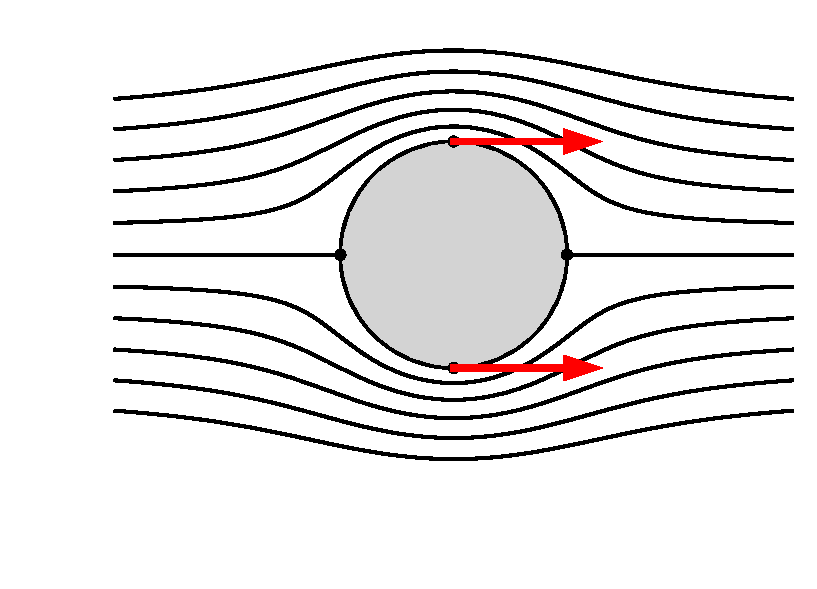
\includegraphics[width=0.7\linewidth]{Figures/Chapter3/fig_cylinder_stream}
\caption{The streamlines for the flow around the cylinder.  Note that there are stagnation points upstream and downstream of the cylinder ($\phi = 0$ and $\phi = \pi$), and the fluid has greatest velocity at the top and bottom ($\phi = \pi2$ and $\phi = 3\pi/2$).}
\label{fig_cyl_streamlines}
\end{figure}

Let's examine the flow in a little more detail.  Note that, as necessary, $u_s=0$ at $s=a$.  On the boundary, the flow is purely angular, with speed 
\[
u_\phi = -2U \sin \phi \quad \text{at} \quad s=a.
\]
At $\phi = 0$ and $\phi = \pi$, then $u_\phi = 0$ and there is a stagnation point there (see Figure \ref{fig_cyl_streamlines}).  There is a maximum speed at $\phi = \pi/2$ and $\phi = 3\pi/2$ of
\[
u_{\phi, \text{max}} = 2U \quad \text{at} \quad s=a.
\]

What about the pressure in the fluid?  Well, we could apply Euler's equation to find it, but Bernoulli's principle provides a shortcut.  Since the flow is irrotational, $\grad H = 0$ and $H = p/\rho + \tfrac{1}{2} \uu^2 + gz = $ constant everywhere in the fluid.  In our analysis, though, we'll neglect the gravity term; we're only looking at the $(s, \phi)$ dependence of the pressure here, and gravity will only impose an overall vertical pressure gradient.

Let's first evaluate $H$ at infinity, where $\uu = (U,0,0)$ and we'll label the pressure $p_\infty$.  Then
\[
H = \frac{p_\infty}{\rho} + \tfrac{1}{2} U^2.
\]
Elsewhere in the fluid, it's
\[
H = \frac{p(s, \phi)}{\rho} + \tfrac{1}{2} \uu^2,
\]
where
\[
\uu^2 = \uu \cdot \uu = u_s^2 + u_\phi^2 = U^2 \left( 1 + \frac{a^4}{s^4} - 2\frac{a^2}{s^2} \cos 2\phi \right)
\]
(that last step required some algebra to clean up, though).  Since $H$ is constant, we have
\[
\frac{p(s, \phi)}{\rho} + \tfrac{1}{2} U^2 \left( 1 + \frac{a^4}{s^4} - 2\frac{a^2}{s^2} \cos 2\phi \right) = \frac{p_\infty}{\rho} + \tfrac{1}{2} U^2.
\]
Rearranging gives the pressure,
\begin{equation}
p(s, \phi) = p_\infty + \tfrac{1}{2} \rho \frac{a^2}{s^2} U^2 \left( 2 \cos 2\phi - \frac{a^2}{s^2} \right).
\end{equation}
Figure \ref{fig_cyl_pressure} shows the pressure around the cylinder; there is a region of high pressure at $\phi = 0$ and $\phi = \pi$, with low pressure at $\phi = \pi/2$ and $\phi = 3\pi/2$.  Not surprisingly, this is opposite the fluid velocity -- expected, since Bernoulli's theorem holds here.

\begin{figure}[t]
\centering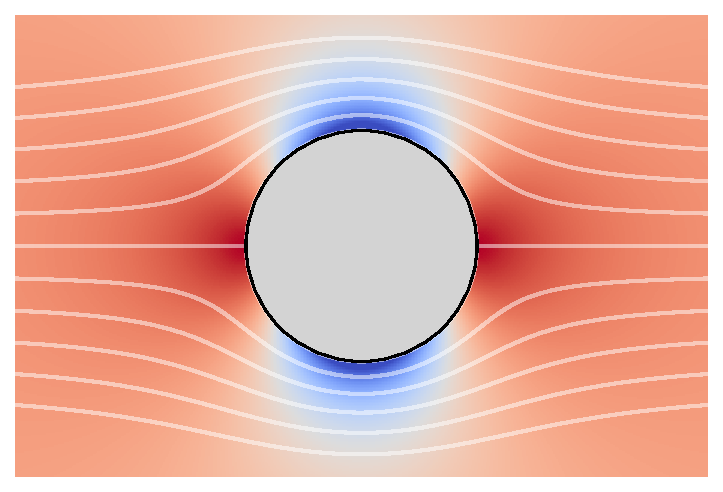
\includegraphics[width=0.8\linewidth]{Figures/Chapter3/fig_cylinder_pressure}
\caption{The pressure field of fluid flowing past a cylinder.  The dark red regions are areas of high pressure, while the blue areas are low pressure.  The streamlines are shown as well.}
\label{fig_cyl_pressure}
\end{figure}


\subsection{The Stream Function}

Let's take a break from thinking about irrotational flow for a moment, and instead consider flow that is incompressible (it's important to note that the velocity potential $\varphi$ doesn't require incompressibility to describe flow, just irrotationality).  We'll impose the further restriction that it is also two dimensional only -- so $\vec{u} = [u(x, y, t), v(x, y, t), 0]$.  In this case, we'll define the \emph{stream function} $\psi$ by
\begin{equation}
\label{eq_stream_def}
\boxed{
\vec{u} = \curl (\psi \, \unit{z}).
}
\end{equation}

Why this particular function?  Well, consider it in Cartesian coordinates,
\begin{equation}
u = \dfdx{\psi}{y} \quad \text{and} \quad v = - \dfdx{\psi}{x}.
\end{equation}
With this definition, the incompressibility equation is automatically satisfied:
\[
\grad \cdot \uu = \dfdx{u}{x} + \dfdx{v}{y} = \dfdx{}{x} \left( \dfdx{\psi}{y} \right) + \dfdx{}{y} \left( - \dfdx{\psi}{x} \right) = 0,
\]
since the order of the derivatives doesn't matter.  Compare this with the velocity potential:  it ensures irrotational flow, while the stream function ensures incompressible flow, at the cost of requiring it to be two dimensional.  By the way, in cylindrical coordinates, this definition becomes
\begin{equation}
\label{eq_stream_cyl}
u_s = \frac{1}{s} \dfdx{\psi}{\phi} \quad \text{and} \quad u_\phi = - \dfdx{\psi}{s}.
\end{equation}

You might be wondering why the stream function has that particular name -- and it turns out the reason is one of its most useful features.  Note that
\[
(\vec{u} \cdot \grad ) \psi = u\dfdx{\psi}{x} + v\dfdx{\psi}{y} = \dfdx{\psi}{y} \dfdx{\psi}{x} + \left( -\dfdx{\psi}{x} \right) \dfdx{\psi}{y} = 0.
\]
Remember what this means from Section \ref{sec_tot_deriv} -- that $\psi$ is constant on streamlines; hence the name.  If we know the stream function $\psi$, we'll now be able to easily plot the streamlines:  just set $\psi$ to a constant.  Different values of the constant will give you different streamlines.


\begin{example}[Flow past a stagnation point]
\label{ex_stag_psi}
Let's continue on from Example \ref{ex_stag_pot} and find the stream function for the flow
\[
\vec{u} = [\alpha x, -\alpha y, 0],
\]
which is incompressible (feel free to check) and obviously two dimensional.  From $u = \partial \psi / \partial y$ we get
\[
\dfdx{\psi}{y} = \alpha x,
\]
which integrates to 
\[
\psi(x, y) = \alpha x y + f(x),
\]
where $f(x)$ is some possible function of $x$.  From $v = -\partial \psi / \partial x$, we end up with something similar after integrating,
\[
\psi(x, y) = \alpha x y + g(y),
\]
where again $g(y)$ is our integration ``constant.''  Now, comparing the two equations for $\psi$, it's clear that we must have
\begin{equation}
\psi(x, y) = \alpha x y.
\end{equation}

Streamlines for this flow can be found from setting $\psi$ to a constant, which we'll call $k$:
\[
\psi = \alpha x y = k,
\]
or
\[
y = \frac{k}{\alpha x} = \frac{c}{x},
\]
where $c = k/\alpha$.  This exactly matches the equation we found back in Example \ref{ex_stag_stream} for the streamlines of a flow about a stagnation point.
\end{example}



\begin{example}[Line vortex flow]
\label{ex_vortex_psi}
For the line vortex flow, from Example \ref{ex_pot_vortex} with
\[
\uu = \frac{\Gamma}{2\pi s} \, \hat{\phi},
\]
the process to finding the stream function is similar, but we have to use cylindrical coordinates.  From equation (\ref{eq_stream_cyl}), we get
\[
u_s = 0 = \frac{1}{s} \dfdx{\psi}{\phi} \quad \text{and} \quad u_\phi = \frac{\Gamma}{2\pi s} = -\dfdx{\psi}{s}.
\]
From the first equation we just find that $\psi$ has no $\phi$ dependence, and from the second, upon integrating, we get
\[
\psi(s, \phi) = -\frac{\Gamma}{2\pi} \ln s.
\]

Once again we can find the streamlines from the stream function by setting $\psi$ to a constant (call it $k$ again).  Doing so and solving for $s$ gives
\[
s = e^{-2\pi k / \Gamma} = \text{constant}.
\]
This makes sense, since we know this is circular flow -- the streamlines are circles of constant radius $s$.
\end{example}

Like the velocity potential, the stream function satisfies Laplace's equation as long as the flow is both incompressible and irrotational -- although here we need the additional constraint of two dimensional flow as well.  The proof is straightforward: start with the condition for irrotational flow, $\curl \uu = \vec{0}$, and substitute in the definition of the stream function from equation (\ref{eq_stream_def}) to get
\[
\curl [ \curl (\psi \, \unit{z}) ] = \vec{0}.
\]
But we can expand the curl of a curl as
\[
\curl [ \curl (\psi \, \unit{z}) ] = \grad [\grad \cdot (\psi \, \unit{z})] - \nabla^2 (\psi \, \unit{z}) = \vec{0},
\]
and, for two dimensional flow, the first term goes to zero, so we're left with
\begin{equation}
\boxed{
\nabla^2 \psi = 0.
}
\end{equation}
So both the velocity potential $\varphi$ and the stream function $\psi$ satisfy Laplace's equation for two dimensional, irrotational, incompressible flow.  Although not every problem in fluid dynamics satisfies these restrictions, many do, and we'll exploit this in the next chapter to investigate some interesting and complex situations.




\section*{Problems}
\addcontentsline{toc}{section}{Problems}
\markright{Problems}%

\begin{problem}[Yet more vector calculus]
\label{prob_vc3}
Show that, for any vector field $\symbfup{v}$, you can write
\[
(\symbfup{v} \cdot \grad ) \symbfup{v} = (\curl \symbfup{v}) \times \symbfup{v} + \grad(\tfrac{1}{2} \symbfup{v}^2).
\]
\end{problem}

\begin{problem}[Please, no more vector calculus]
\label{prob_vc4}
Show that, for any two vector fields $\symbfup{F}$ and $\symbfup{G}$, you can write
\[
\curl (\symbfup{F} \times \symbfup{G}) = (\symbfup{G} \cdot \grad) \symbfup{F} - (\symbfup{F} \cdot \grad) \symbfup{G} + \symbfup{F} (\symbfup{\nabla} \cdot \symbfup{G}) - \symbfup{G} (\symbfup{\nabla} \cdot \symbfup{F})
\]
\end{problem}


\begin{problem}[The Rankine Vortex as a Model for Hurricanes]

\begin{figure}
\centering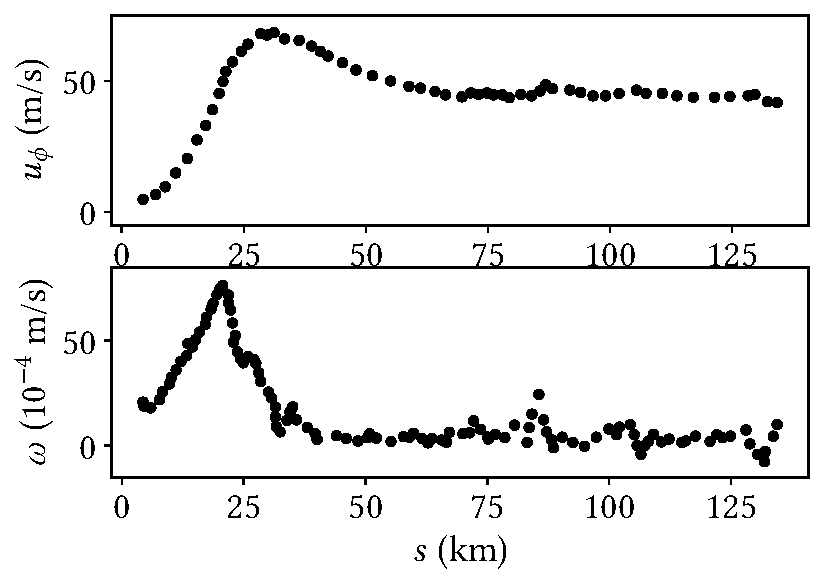
\includegraphics[width=0.8\linewidth]{Figures/Chapter3/fig_hurricane_data}
\caption{The azimuthal wind speed $u_\phi(s)$ and vorticity $\omega(s)$ for Hurricane Katrina.  Data from Corbosiero, K. ``Advanced Research WRF high resolution simulations of the inner core structures of Hurricanes Katrina, Rita, and Wilma (2005).'' \emph{Proceedings, 8th Annual WRF Users Workshop, Boulder, CO, NCAR.} 2007.}
\label{fig_hurricane_data}
\end{figure}

A Rankine vortex is defined by the flow (in cylindrical coordinates)
\[
\symbfup{u}  = \left\{
 \begin{array}{l l}
    \Omega s \, \hat{\phi} & \quad \text{if $s < a$}\\
   \frac{\Omega a^2}{s} \, \hat{\phi} & \quad \text{if $s>a$,}
  \end{array} \right.
\]
where $\Omega$ and $a$ are constants (related to the wind speed and size of the ``core,'' respectively).  It serves as a useful model for a number of weather and atmospheric conditions, such as hurricanes, mesocyclones, and tornadoes.  

(a) Plot the wind speed as a function of distance, and calculate and plot the vorticity.

(b) To decide whether it is a useful model for hurricanes, I've provided azimuthal wind speed data and vorticity data for Hurricane Katrina, which devastated New Orleans and the surrounding area in 2005, in Figure \ref{fig_hurricane_data} (you can extract this data using online tools such as PlotDigitizer). Use the Rankine vortex (RV) to model this hurricane; what values of $\Omega$ and $a$ give you the best fit?  Does the RV model the vorticity with those parameters as well?  Can you make any conclusions about how well the model does (e.g., is it better in some regions versus others?)

(c) Calculate the pressure throughout the hurricane and find the difference in pressure between r = 0 (the eye of the hurricane) and $s \to \infty$ (outside the storm).

(d) Finally, calculate the shape of the free surface (i.e., where the pressure is atmospheric). Plot the surface, and compare this with photos of Katrina -- how does it look?



\end{problem}



\begin{problem}[The force on a cylinder]
\label{prob_force1}
We've already calculated the pressure in the fluid around a cylinder in Section \ref{sec_cylinder}, so it's a short leap to find the total force exerted on the cylinder by the fluid.

Consider Figure \ref{fig_cylinder_force}:  the force (per unit length of the cylinder) on a small angular section of size $a \, d\phi$ is
\[
d\textbf{F} = - p a \, d\phi \, \hat{n}.
\]
Using this, show the total force on the cylinder is zero.  This is called \emph{D'Alembert's paradox} -- there's no drag on the cylinder, despite very obvious physical evidence to the contrary.  Does it make sense that the fluid exerts no force at all on the cylinder as it flows past?  Discuss.

\begin{figure}[t]
\centering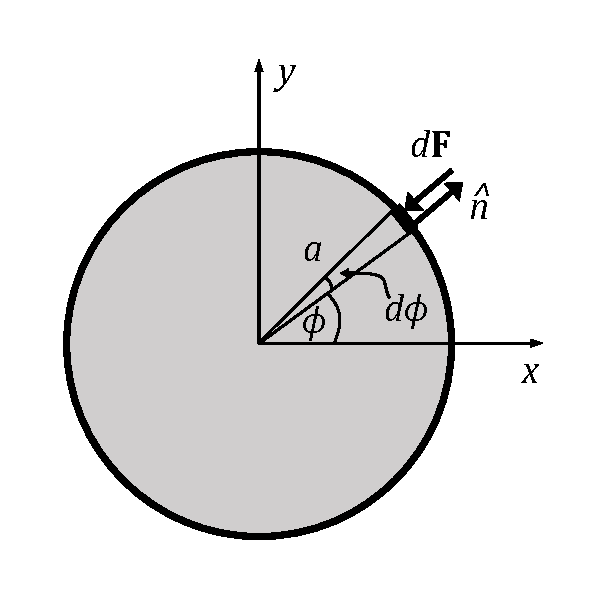
\includegraphics[width=0.5\linewidth]{Figures/Chapter3/fig_cyl_force}
\caption{The force on a small angular section of the cylinder.  The force is opposite the normal vector $\hat{n}$.}
\label{fig_cylinder_force}
\end{figure}
\end{problem}


\begin{problem}[Uniform Flow]
\label{prob_uniform_pot}
Consider two dimensional flow that is constant with speed $U$ and flows in a direction at an angle $\alpha$ with respect to the $x$ axis (see Figure \ref{fig_uniform_flow_angle}).  

(a) Find the velocity potential $\varphi(x, y)$.

(b) Find the stream function $\psi(x, y)$.

\begin{figure}[t]
\centering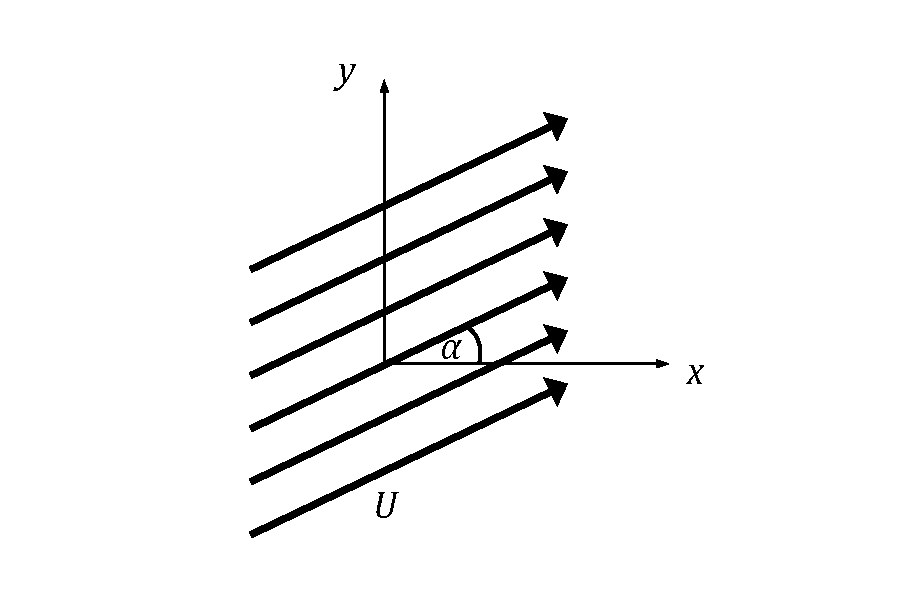
\includegraphics[width=0.7\linewidth]{Figures/Chapter3/fig_uniform_flow_angle}
\caption{A constant flow that makes an angle $\alpha$ with the $x$ axis.}
\label{fig_uniform_flow_angle}
\end{figure}
\end{problem}

\begin{problem}[Line source and sink]
\label{prob_line_source}
Consider the two dimensional flow 
\begin{equation}
\uu = \frac{Q}{2\pi s} \, \unit{s},
\end{equation}
where $Q$ is a constant (you might want to compare the form of this flow to the line vortex).  This is called a \emph{line source} if $Q$ is positive and a \emph{line sink} if it's negative.

(a) Produce a vector plot for the flow.

(b) Find the  velocity potential $\varphi(s, \phi)$.

(b) Find the stream function $\psi(s, \phi)$.
\end{problem}

\begin{problem}[Plotting streamlines]
Consider the two dimensional flow
\[
\uu = [2x+3, -2y].
\]

(a) Show that the flow is irrotational and incompressible.

(b) Find the stream function $\psi(x, y)$ and plot the streamlines.
\end{problem}
